\section{Desenvolvimento do Código}

\subsection{Configurações Iniciais}

Para desenvolver o código, usamos o Visual Studio Code (VSCode) com a extensão PlatformIO. Na página inicial da extensão, criamos um novo projeto utilizando a placa "Espressif ESP32 Dev Module" e o framework "Arduino".

Começamos definindo a taxa de atualização do monitor e iniciando o módulo Serial para poder visualizar informações no Terminal.

\begin{lstlisting}
// platformio.ini
monitor_speed = 9600

// main.cpp
void setup(){
    Serial.begin(9600);
}
\end{lstlisting}

\subsection{Biblioteca ThingSpeak}

Para enviar dados para o ThingSpeak, precisamos instalar a sua biblioteca. Voltamos para a página inicial da extensão Platform IO e acessamos a aba \textit{Libraries}. Pesquisamos por "ThingSpeak" e adicionamos a biblioteca ao projeto que estamos trabalhando.

\begin{figure}[H]
    \centering
    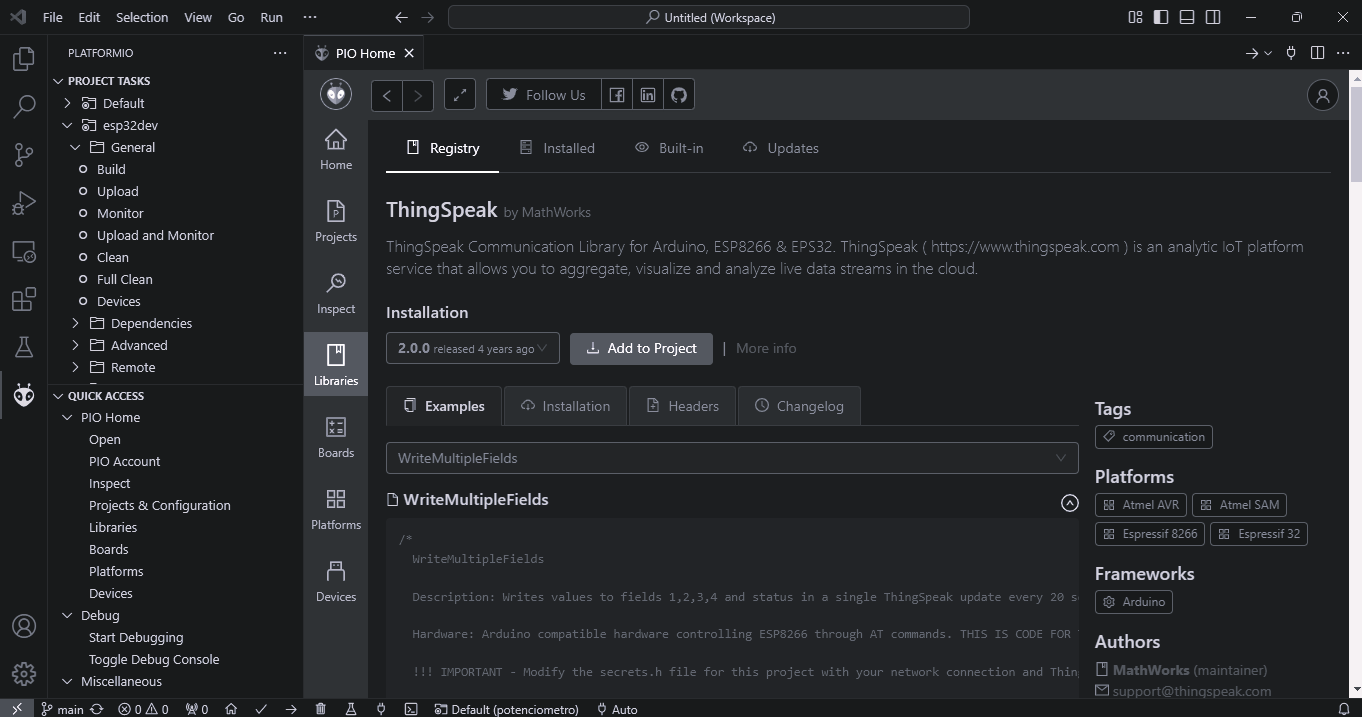
\includegraphics[width=0.5\linewidth]{img/platformio-thingspeak.png}
    \caption{Tela de instalação da biblioteca Thingspeak.}
    \label{fig:platformio-thingspeak}
\end{figure}

Feito a instalação, importamos a biblioteca. Aproveitamos para importar também a biblioteca Wifi que será necessária.
\begin{lstlisting}
#include <Wifi.h>
#include "ThingSpeak.h"
\end{lstlisting}

\subsection{Configuração em Setup}

De primeiro momento, definimos uma constante para representar o pino vermelho do LED RGB e criamos uma variável \textit{client} da classe WifiClient.

\begin{lstlisting}
#define LED_RED 22

WiFiClient client;
\end{lstlisting}

Na função \textit{setup}, configuramos o módulo Wifi para que funcione em modo estacionário com o método \textit{mode}, iniciamos o módulo do ThingSpeak passando como parâmetro a variável \textit{client}, definimos o modo do pino vermelho do LED como modo de saída.

\begin{lstlisting}
void setup() {
    // ...
    WiFi.mode(WIFI_STA);
    ThingSpeak.begin(client);
    pinMode(LED_RED, OUTPUT);
}
\end{lstlisting}

\subsection{Conectando ao Wi-Fi}

Na função \textit{loop}, começamos iniciando o módulo Wi-Fi. Com o método \textit{status}, conferimos se o dispositivo já está conectado a um rede Wi-Fi, se não estiver, usamos o método \textit{begin} e passamos as credenciais da rede para realizar a conexão. Adicionamos um laço \textit{while} que só termina quando o método \textit{status} retorna um sinal positivo de que a conexão foi feita.

\begin{lstlisting}
if (WiFi.status() != WL_CONNECTED) {
    Serial.print("Attempting to connect");
    
    while (WiFi.status() != WL_CONNECTED) {
        Serial.print(".");
        WiFi.begin(SSID, PASSWORD);
        delay(5000);
    }
    
    Serial.println("\nConnected.");
}
\end{lstlisting}

\subsection{Potenciômetro}

Para ler o potenciômetro, definimos uma constate para representar o seu pino. Também criamos uma variável do tipo inteiro para guardar os valores.
\begin{lstlisting}
#define POTENCIOMETER 34

int potenciometer;
\end{lstlisting}

Não é necessário configurar o modo do pino. Voltando para \textit{loop}, usamos a função \textit{analogRead} para ler o pino do potenciômetro. Os pinos de entrada analógica possuem resolução de 12 bits, então os valores vão de 0 à 4095. Atribuímos o valor à variável que criamos e imprimimos no monitor.

\begin{lstlisting}
potenciometer = analogRead(POTENCIOMETER);
Serial.print("Resolucao:");
Serial.println(potenciometer);
\end{lstlisting}

\subsection{Defininindo a tensão e a luminosidade}
Nessa parte, utilizamos o valor que o potenciômetro nos dá para calcular a tensão e definir a luminosidade do LED. Primeiro, criamos variáveis para guardar esses valores.

\begin{lstlisting}
float tension;
int ledTension;
\end{lstlisting}

Para calcular a tensão no pino, é preciso entender que a tensão dos pinos vão de 0 \textit{volts} até 3.3 \textit{volts}. Fazendo uma regra de três junto com os valores do potenciômetro, conseguimos o valor da tensão desse modo:

$$\text{tensão} = \text{potenciômetro} * \frac{3.3}{4095}$$

Aplicamos a fórmula e imprimimos o valor no monitor.

\begin{lstlisting}
tension = potenciometer * (3.3 / 4095);
Serial.print("Tensao: ");
Serial.println(tension);
\end{lstlisting}

O método é exatamento o mesmo para definir a luminosidade do LED RGB. Os valores do \textit{duty circle} vão de 0 até 255. Substituindo, a fórmula é:

$$\text{tensão no led} = \text{potenciômetro} * \frac{255}{4095}$$

Novamente, aplicamos a fórmula no código e imprimimos o valor. E também, utilizamos a função \textit{analogWrite} para definir a luminosidade.

\begin{lstlisting}
ledTension = potenciometer * (255.0 / 4095.0);
analogWrite(LED_RED, ledTension);
Serial.print("Tensao no Led: ");
Serial.println(ledTension);
\end{lstlisting}

\subsection{Publicando no ThingSpeak}

Conectar ao ThingSpeak requer a chave de API que ele gera quando o canal é criado. Copiamos ela para código. Guardamos também a quantidade de canais que foram criados, que no nosso caso, foi apenas um.

\begin{lstlisting}
unsigned long myChannelNumber = 1;
const char *myWriteAPIKey = "";
\end{lstlisting}

Para enviar os dados para o gráfico do \textit{ThingSpeak}, usamos a função \textit{writeField} do módulo. Ela aceita o número do canal, o número do campo, o valor que queremos publicar e chave da API do ThingSpeak.

\begin{lstlisting}
int x = ThingSpeak.writeField(myChannelNumber, 1, tension, myWriteAPIKey);
\end{lstlisting}

A função retorna um valor conferir se a publicação foi um êxito ou não. Se for, o valor retorna é 200.

\begin{lstlisting}
if (x == 200) {
    Serial.println("Channel update successful.");
} else {
    Serial.println("Problem updating channel. HTTP error code " + String(x));
}
\end{lstlisting}

Como estamos acessando uma API, é interessante definir um \textit{delay}. Criamos essas variáveis para guardar o tempo de execução e o \textit{delay}.

\begin{lstlisting}
unsigned long lastTime = 0;
unsigned long timerDelay = 2500;
\end{lstlisting}

Em \textit{loop}, colocamos todo o código escrito dentro um \textit{if} condicional que só deixará o fluxo entrar quando já estiver passado o tempo de \textit{delay}. Utilizamos a função \textit{millis} que retorna o tempo de execução em milisegundos.\newpage

\begin{lstlisting}
if ((millis() - lastTime) > timerDelay) {
    // ...
}
\end{lstlisting}

Precisamos atualizar a variável \textit{lastTime} toda vez que o código é executado.

\begin{lstlisting}
if ((millis() - lastTime) > timerDelay) {
    // ...
    
    lastTime = millis();
}
\end{lstlisting}